\chapter{Introduction}
Focal adhesions (FA) are macromolecular protein complexes which act as a connection hub between the cell, especially the cytoskeleton, and the extracellular matrix (ECM). They enable the cell to exert tension forces, but can also transduce mechanical stimuli from the ECM to the inside of the cell and integrate this information. One important protein associated to FAs is the focal adhesion kinase (FAK). FAK occurs in several signalling pathways and is a key player in integrating extracellular stimuli. It is of large interest not least because often an overexpression of FAK can be found in cancer cells, and understanding the activation processes and dynamics of FAK could give rise to new cancer treatments \autocite{cancerFAK}.
\section{Structure of FAK}
FAK consists of four domains: (i) a FERM (4.1 protein, ezrin, radixin and moesin) domain at the N-terminus, (ii) a tyrosine kinase, (iii) a proline-rich region and (iv) a focal adhesion targeting (FAT) domain at the C-terminus (see \Cref{intro:fak}).\\
FERM is a common protein domain which links proteins to membranes by binding to various phospholipids \autocite{fermdomain} and consists of three subdomains: F1, F2 and F3. In the F2 subdomain, a basic patch ($^{216}$KAKTLRK$^{222}$) can be found, which is a prominent binding site for phosphatidylinositol-4,5-bisphosphate (\pip).\\
The kinase consists of a C-lobe, an activation loop and an N-lobe. Catalytic activity of the kinase is mainly regulated by the phosphorylation of \acid{Y}{576}{} and \acid{Y}{577}, which are located in the activation loop \autocite{tyrosinePhosphor}. The kinase also provides binding sites for \pip{}. One is located next to the basic patch of the FERM domain, but others (namely \acid{R}{508}, \acid{R}{514}, \acid{K}{515}, \acid{K}{621} and \acid{K}{627}) can be found on the side of the kinase \autocites{pap002}{pap002Exp}.\\
The FERM domain and the kinase are connected by a linker region. In contrast to other kinase domains, the main autophosphorylation site of FAK, \acid{Y}{397}, can be found in this region and not in the kinase itself \autocite{pap001}.\\
The FAT domain is linked to the kinase by a flexible proline-rich region. FAT links to FAs by interacting with talin and paxillin which are integrin-associated proteins \autocite{fatdomain}.
%
%
%
\begin{figure}
	\centering
	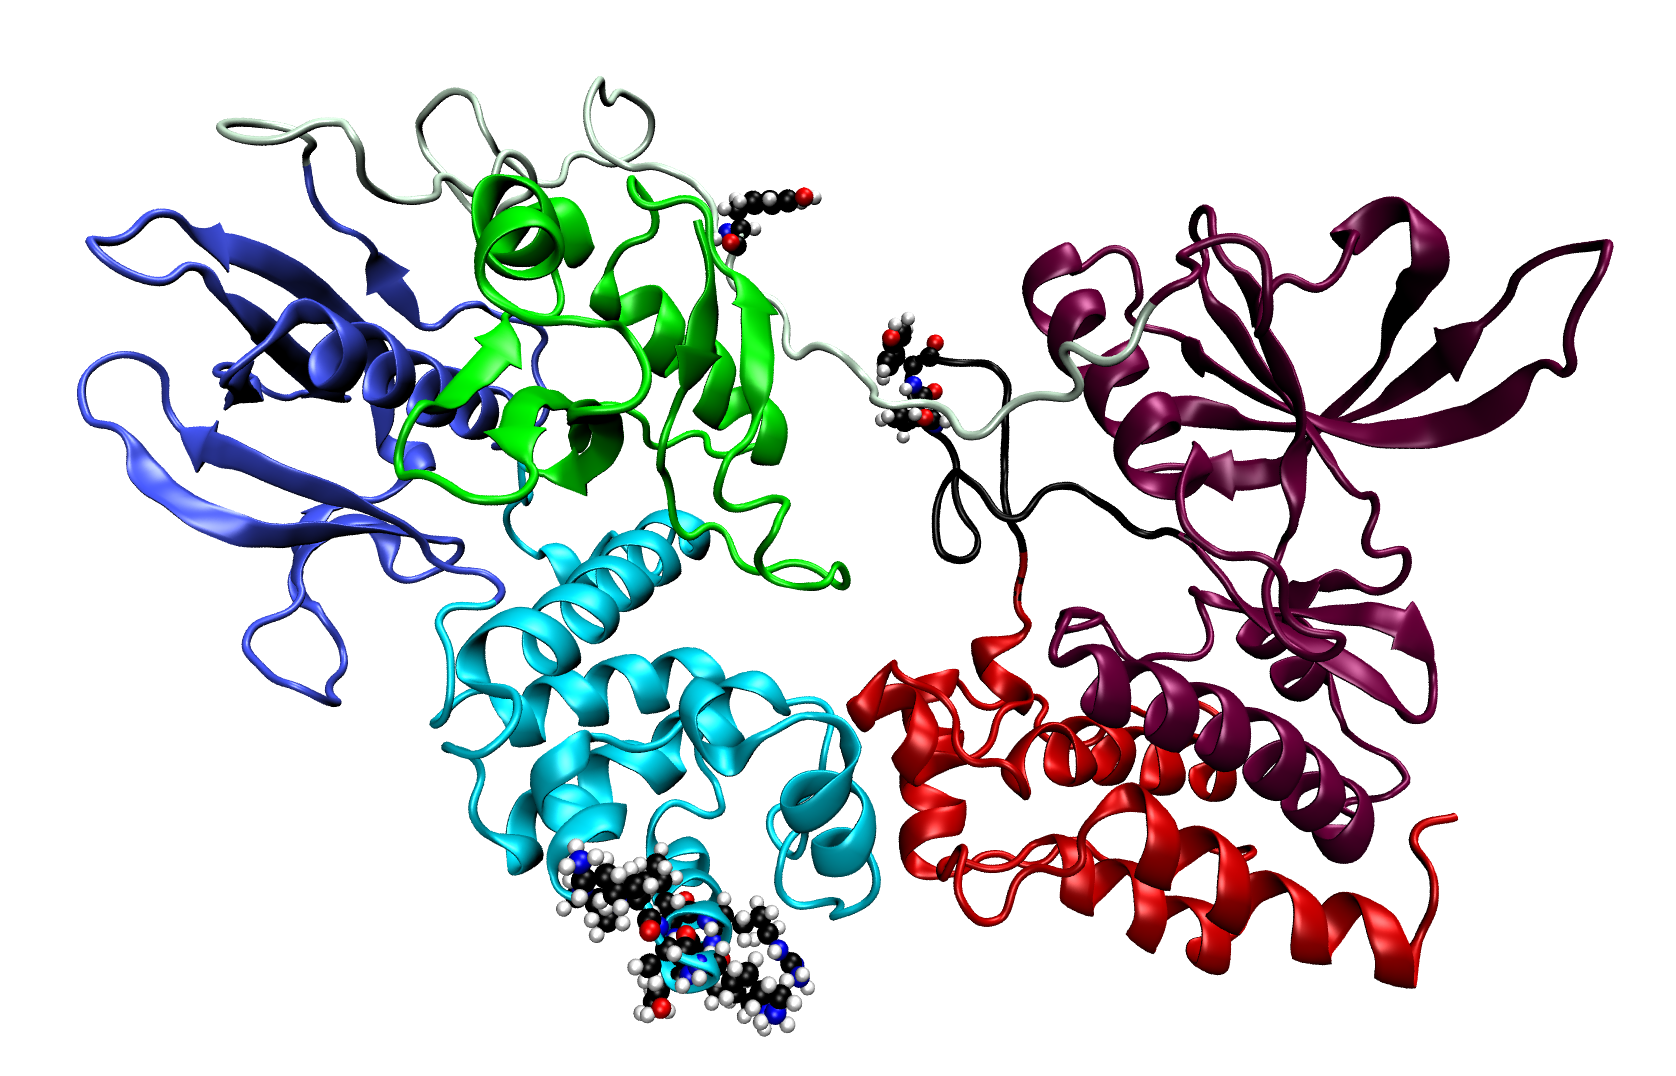
\includegraphics[height=6cm]{figures/introduction/fak}
	\nicecaption{Structure of FAK}{The FERM domain, consisting of F1 (green), F2 (iceblue) and F3 (blue), and the kinase, consisting of N-lobe (violet), activation loop (black) and C-lobe (red), are connected via the linker region (white). The basic patch (in F2), \acid{Y}{397} (in the linker) and \acid{Y}{567}, \acid{Y}{577} (in the activation loop) are shown in atomistic representation.}
	\label{intro:fak}
\end{figure}
%
%
%
\section{\pip{} binding and activation}
It is known that integrin signalling due to cell adhesion triggers activation of FAK and that \pip{} is an important mediator in this signalling pathway. FAK interacts in several ways with \pip{}, which is discussed in the following.\\
\\
In the autoinhibited conformation, the FERM domain shields the active site of the kinase. Therefore, an activation of FAK requires the dissociation of the FERM and the kinase \autocite{structFAK}.\\
\pip{} is a phospholipid which is locally generated in FAs due to integrin signalling \autocite{pip2LocalGeneration}. Its charge depends strongly on the pH, but at physological conditions a net charge of -4 is the preferred state. However, in presence of basic amino acids (Arg, Lys), the deprotonated state gets promoted, resulting in a net charge of -5 \autocite{pip2_minus5}. The electrostatic binding of \pip{} to the basic patch in the F2 subdomain results in allosteric changes, which also influence the interface between the F1 subdomain and the N-lobe. Moreover, the linker region gets less strongly bound, which promotes autophosphorylation of \acid{Y}{397}. Because the \pip{} binding alone has no effect on the catalytic activity, which suggests that the FERM domain is still associated to the kinase \autocites{pap001}{pap003}. For activation, an additional stimulus, either biochemical or mechanical, is needed.\\
\\
Autophosphorylation of \acid{Y}{397} is an important step in FAK activation. Once this site is phosphorylated, it becomes a suitable binding site for SH2 or SH3, which are subdomains of proteins of Src family tyrosine kinases. Due to the conformational changes induced by \pip{}, this kinase has access to \acid{Y}{576} and \acid{Y}{577}. As said, the phosphorylation of these residues makes FAK fully active, resulting in dissociation of the FERM domain and the kinase \autocite{pap001}. Once the activation loop is phosphorylated, the FERM domain cannot inhibit the kinase any more. Therefore, a dephosphorylation is required to downregulate FAK activity \autocite{structFAK}.\\
\\
Mechanical forces can lead to dissociation of the FERM domain from the kinase as well. Forces acting on the FAT domain are transduced to the FERM-kinase interface because the linker is connected to the kinase, while the FERM domain is anchored onto a \pip{} containing membrane. These forces can lead to activation of FAK. In that way, it is acting as a mechanical sensor \autocite{pap004}.\\
\\
The binding sites for \pip{} on the side of the kinase were identified via computer simulations \autocite{pap002} and have been confirmed recently in experiments \autocite{pap002Exp}. The findings from \textcite{pap002Exp} show that these residues are required for catalytic activity of the kinase, and that they bind to phospholipids \textit{in vivo}. However, since the catalytic activity is not regulated by \pip{} alone, this binding was hypothesized to act as a stabilisation of the active state only \autocite{pap002Exp}.
\section{Dimerization and clustering}
\label{intro:clustering}
Experimental findings suggest that self-association of FAK, such as dimerization or clustering, can trigger autophosphorylation of \acid{Y}{397} \autocites{transAuto}{dimersVsClusters}.\\
\\
The FERM domain induces a dimerization of FAK by interacting with the FERM domain of a neighbouring FAK molecule. The interaction emerges around \acid{W}{266} in the connected FERM domains and is stabilised by an interaction of the FAT domain with the basic patch of the other FERM domain, respectively. \pip{} is not required for the dimerization of the FERM domains. However, an enriched FAK concentration is needed to observe FAK dimers in cells, which is the case at FAs. It is still unclear how the dimer could be stabilised at membranes, where the basic patch is also required for ligand binding \autocite{fakdimers}.\\
\\
\pip{} does not only induce conformational changes, but also clustering of several FAK molecules on the membrane \textit{in vitro} \autocite{pap001}. In contrast to dimers, clusters of FAK molecules can trigger additional biochemical stimuli \autocite{dimersVsClusters} and may play an important role in the scaffolding function of FAK for FAs \autocite{pap001}.
